\documentclass[]{article}
\usepackage{lmodern}
\usepackage{amssymb,amsmath}
\usepackage{ifxetex,ifluatex}
\usepackage{fixltx2e} % provides \textsubscript
\ifnum 0\ifxetex 1\fi\ifluatex 1\fi=0 % if pdftex
  \usepackage[T1]{fontenc}
  \usepackage[utf8]{inputenc}
\else % if luatex or xelatex
  \ifxetex
    \usepackage{mathspec}
  \else
    \usepackage{fontspec}
  \fi
  \defaultfontfeatures{Ligatures=TeX,Scale=MatchLowercase}
  \newcommand{\euro}{€}
\fi
% use upquote if available, for straight quotes in verbatim environments
\IfFileExists{upquote.sty}{\usepackage{upquote}}{}
% use microtype if available
\IfFileExists{microtype.sty}{%
\usepackage{microtype}
\UseMicrotypeSet[protrusion]{basicmath} % disable protrusion for tt fonts
}{}
\usepackage[margin=1in]{geometry}
\usepackage{hyperref}
\PassOptionsToPackage{usenames,dvipsnames}{color} % color is loaded by hyperref
\hypersetup{unicode=true,
            pdftitle={Atlas da Radiação Solar da Ilha da Madeira},
            pdfauthor={Ricardo Faria},
            pdfborder={0 0 0},
            breaklinks=true}
\urlstyle{same}  % don't use monospace font for urls
\usepackage{longtable,booktabs}
\usepackage{graphicx,grffile}
\makeatletter
\def\maxwidth{\ifdim\Gin@nat@width>\linewidth\linewidth\else\Gin@nat@width\fi}
\def\maxheight{\ifdim\Gin@nat@height>\textheight\textheight\else\Gin@nat@height\fi}
\makeatother
% Scale images if necessary, so that they will not overflow the page
% margins by default, and it is still possible to overwrite the defaults
% using explicit options in \includegraphics[width, height, ...]{}
\setkeys{Gin}{width=\maxwidth,height=\maxheight,keepaspectratio}
\setlength{\parindent}{0pt}
\setlength{\parskip}{6pt plus 2pt minus 1pt}
\setlength{\emergencystretch}{3em}  % prevent overfull lines
\providecommand{\tightlist}{%
  \setlength{\itemsep}{0pt}\setlength{\parskip}{0pt}}
\setcounter{secnumdepth}{5}

%%% Use protect on footnotes to avoid problems with footnotes in titles
\let\rmarkdownfootnote\footnote%
\def\footnote{\protect\rmarkdownfootnote}

%%% Change title format to be more compact
\usepackage{titling}

% Create subtitle command for use in maketitle
\newcommand{\subtitle}[1]{
  \posttitle{
    \begin{center}\large#1\end{center}
    }
}

\setlength{\droptitle}{-2em}
  \title{Atlas da Radiação Solar da Ilha da Madeira}
  \pretitle{\vspace{\droptitle}\centering\huge}
  \posttitle{\par}
  \author{Ricardo Faria}
  \preauthor{\centering\large\emph}
  \postauthor{\par}
  \predate{\centering\large\emph}
  \postdate{\par}
  \date{2016-03-22}



% Redefines (sub)paragraphs to behave more like sections
\ifx\paragraph\undefined\else
\let\oldparagraph\paragraph
\renewcommand{\paragraph}[1]{\oldparagraph{#1}\mbox{}}
\fi
\ifx\subparagraph\undefined\else
\let\oldsubparagraph\subparagraph
\renewcommand{\subparagraph}[1]{\oldsubparagraph{#1}\mbox{}}
\fi

\begin{document}
\maketitle

\section{Introdução}\label{introducao}

\begin{center}\rule{0.5\linewidth}{\linethickness}\end{center}

A realização do estudo do Atlas da Radiação Solar da Ilha da Madeira,
teve iniciativa no estágio do Eng. Ricardo Faria no
\href{http://www.lrec.pt}{LREC}. Este novo Atlas foi realizada com novos
modelos matemáticos, \href{http://www.wrf-model.org}{WRF} para modelação
do clima e o ReSun\textsuperscript{TM} para modelar a distribuição do
recurso solar, em plano horizontal, de modo a identificar de regiões com
maior potencial solar, este último é usado com a colaboração da Empresa
\href{http://megajoule.pt}{Megajoule Inovação}.

\section{Localização e Decrição}\label{localizacao-e-decricao}

\begin{center}\rule{0.5\linewidth}{\linethickness}\end{center}

A região em estudo é a ilha da Madeira, que é a principal ilha do
arquipélago da Madeira, situado no oceano Atlântico, a sudoeste da costa
portuguesa. Encontra-se entre as longitudes -17.3º a -16.64º e latitudes
32.6º a 32.9º. O ponto culminante situa-se no Pico Ruivo, 1.862 m de
altura, a ilha é composta por um perímetro 179.3 km e área de 742.41
km\textsuperscript{2}. O \href{http://www.lrec.pt}{LREC} dispõe de uma
vasta rede de Estações Meteorológicas Automáticas (EMA) distribuidas por
toda a ilha, representada na \ref{fig:ggmap} Fig. 1 e Tab. 1. Reference
(Fenner 2012)

\begin{figure}

{\centering 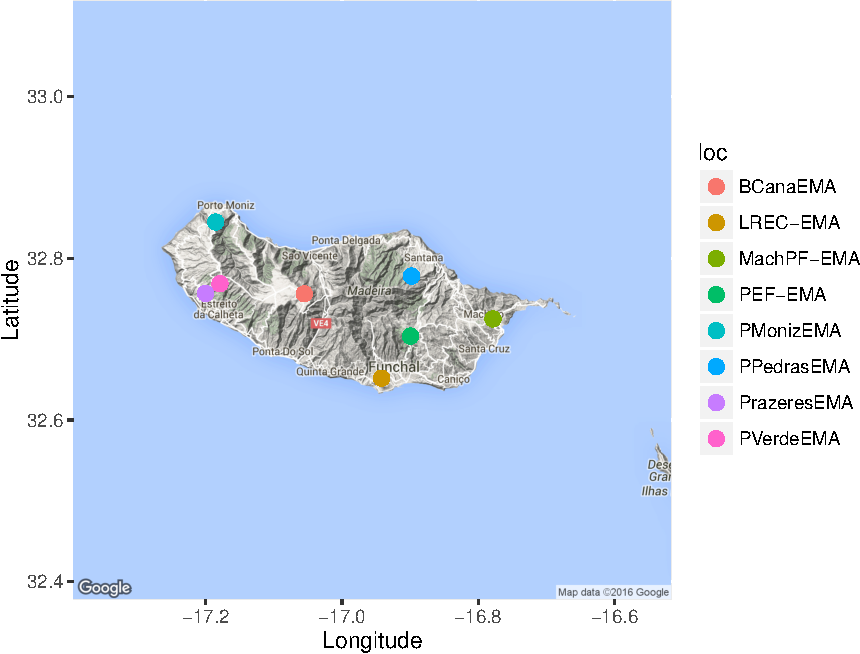
\includegraphics{static_files/figure-latex/ggmap-1} 

}

\caption{Localização da posição das EMAS que pertencem ao LREC}\label{fig:ggmap}
\end{figure}

\begin{longtable}[]{@{}lrr@{}}
\caption{Dados das EMAS}\tabularnewline
\toprule
loc & lat & lon\tabularnewline
\midrule
\endfirsthead
\toprule
loc & lat & lon\tabularnewline
\midrule
\endhead
BCanaEMA & 32.75621 & -17.05530\tabularnewline
LREC-EMA & 32.65179 & -16.94184\tabularnewline
MachPF-EMA & 32.72515 & -16.77819\tabularnewline
PEF-EMA & 32.70387 & -16.89922\tabularnewline
PPedrasEMA & 32.77808 & -16.89781\tabularnewline
PVerdeEMA & 32.76864 & -17.17928\tabularnewline
PMonizEMA & 32.84479 & -17.18550\tabularnewline
PrazeresEMA & 32.75673 & -17.20042\tabularnewline
\bottomrule
\end{longtable}

\subsection{Clima}\label{clima}

Devido à sua latitude, a ilha da Madeira apresenta todas as
características de ilha subtropical, caracteristicament a costa Norte
apresenta um clima temperado, enquanto a Sul denota-se mais subtropical.
Em certos pontos da costa sul, as temperaturas médias anuais atingem
valores acima dos 20 graus celsius. A temperatura da água do mar, varia
entre os 26 de verão e os 17 de inverno. Os ventos predominantes são de
oeste a noroeste no inverno, e de nordeste no verão (alíseos). A
precipitação anual varia de 500 mm no sudeste da ilha aos mais de 2000
mm nas encostas norte.

\subsection{Topografia}\label{topografia}

A ilha da Madeira apresenta uma topografia muito montanhosa, com
profundos vales incrustados entre os picos e suas caraterísticas
falésias.

\begin{figure}

{\centering 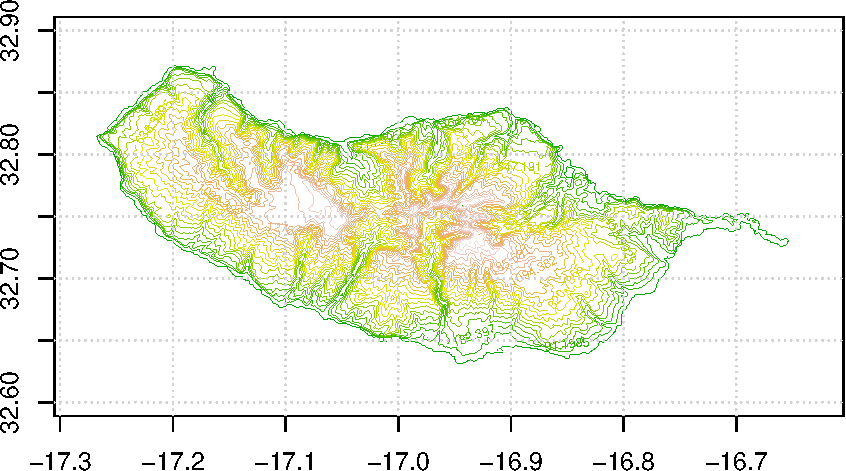
\includegraphics{static_files/figure-latex/topography-1} 

}

\caption{topografia.}\label{fig:topography}
\end{figure}

\section{Metodologia}\label{metodologia}

\begin{center}\rule{0.5\linewidth}{\linethickness}\end{center}

De forma resumida descreve-se a metodologia a usar na elaboração do novo
Atlas Solar do Arquipélago da Madeira: A estimativa do recurso solar
será executada pelo código de simulação ReSun\textsuperscript{TM}
(Pereira et al 2013) na sua variante de modelação, que se encontra
capacitada para modelar os principais factores que afectam a magnitude
do recurso solar, permitindo assim apurar a verdadeira valia da
distribuição do recurso solar de uma forma mais detalhada. A modelação
ReSun\textsuperscript{TM} faz uso de resultados das simulações
meteorológicas WRF (Weather Research \& Forecasting Model), num
procedimento designado de downscaling, que engloba simulações
idealizadas (céu limpo) nos pontos de uma malha de cálculo (mapeamento)
ou pontos discretos de interesse (séries dados). São usadas técnicas de
decomposição da radiação e métodos de interpolação por recurso a
distância efetivas. As simulações a usar na obtenção do Atlas Solar
serão realizadas para um período temporal equivalente a um ano
meteorológico típico, selecionado a partir das Estações Meteorológicas
Automáticas distribuídas pelo arquipélago da Madeira e com auxilio, se
necessário, de dados provenientes de uma análise retrospetiva do
programa MERRA (Modern-Era Retrospective Analysis For Research And
Applications). Os dados das estações serão processados e analisados com
o módulo QC (Solar Data Quality Check) do ReSunTM, onde se fará uma
análise de consistência das medições de radiação global das estações.
Será também realizada uma averiguação da performance do ReSunTM para um
ano a selecionar a partir das medições locais.

\subsubsection{Ano Meteorológico Típico}\label{ano-meteorologico-tipico}

Em termos gerais, a previsão da performance a longo prazo de qualquer
sistema energético solar depende da existência de uma extensa e fiável
base climática local. Teoricamente, esta análise energética deve ser
realizada usando-se vários anos de dados climáticos, o que na maior
parte das vezes não é possível dada a sua inexistência. Isto leva-nos a
ter de recorrer a informação proveniente de bases climáticas de larga
escala obtidas através de modelos de simulação avançados. Contudo, o uso
de períodos extensões para simulação são computacionalmente exigentes,
tornando as análises demasiado morosas e dispendiosas. A variabilidade
inter anual das condições climáticas motiva a necessidade de se derivar
uma base que represente as condições médias de longo prazo num único
ano. Comummente isto é conseguido através de um ano meteorológico típico
(Typical Meterological Year, TMY) constituído pela informação dos 12
meses mais representativos. O método estatístico utilizado para
estimativa do TMY foi o de Filkenstein -- Shafer (FS) devidamente
implementado pela \href{http://megajoule.pt}{Megajoule Inovação}. O
método baseia a seleção dos meses através de uma análise da frequência
cumulativa da média diária dos valores de Radiação Global e Temperatura
para cada um dos meses de um ano civil, Janeiro a Dezembro. De uma forma
resumida, a escolha do ano para cada um dos meses resultará do que
apresentar o menor somatório de erros diários de frequências cumulativas
de um mês em especifico, de um dado ano, face ao longo termo do mês. De
salientar que os erros obtidos para cada uma das variáveis incluídas na
análise do TMY são sujeitas a uma ponderação utilizando-se pesos
diferentes, 70\% e 30\%, radiação solar global e temperatura,
respetivamente.

\subsection{Including Plots}\label{including-plots}

You can also embed plots, for example:

\begin{center}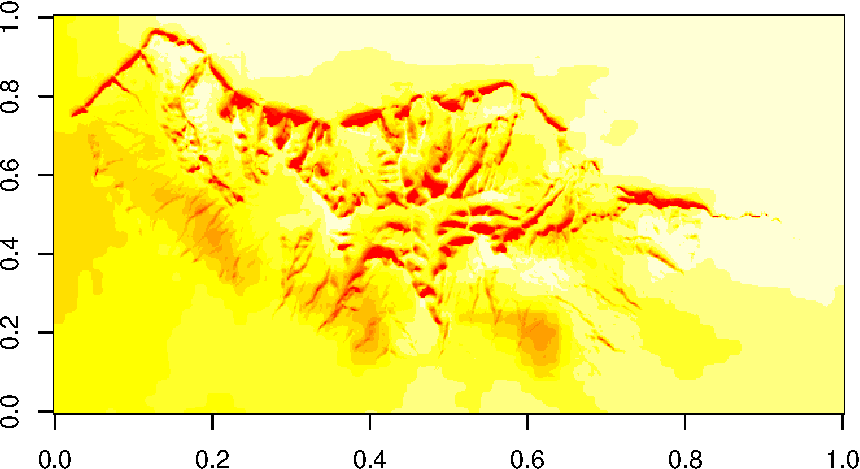
\includegraphics{static_files/figure-latex/pressure-1} \end{center}

Note that the \texttt{echo\ =\ FALSE} parameter was added to the code
chunk to prevent printing of the R code that generated the plot.

\hypertarget{refs}{}
\hypertarget{ref-fenner2012a}{}
Fenner, Martin. 2012. ``One-Click Science Marketing.'' \emph{Nature
Materials} 11 (4). Nature Publishing Group: 261--63.
doi:\href{https://doi.org/10.1038/nmat3283}{10.1038/nmat3283}.

\end{document}
